\chapter{化学测量的统计学}\label{ch:b2:measurement-statistics}

两家实验室测定同一份自来水中的铅，报告结果分别为 9.6 和 \qty{11.2}{\micro g/L}。
饮用水的指导值为 \qty{10}{\micro g/L}。该水是否适于饮用？两家实验室是否真的存在分歧，
还是两次测量的离散所致、实为同一数值？
分析所得的数值若无不确定度便毫无意义，本章给出计算不确定度的工具：
重复测量的统计、不确定度沿计算过程的传递、
最小二乘法定标，以及方法无法检出的下限。
% ledger: who:lead

\begin{omfigure}
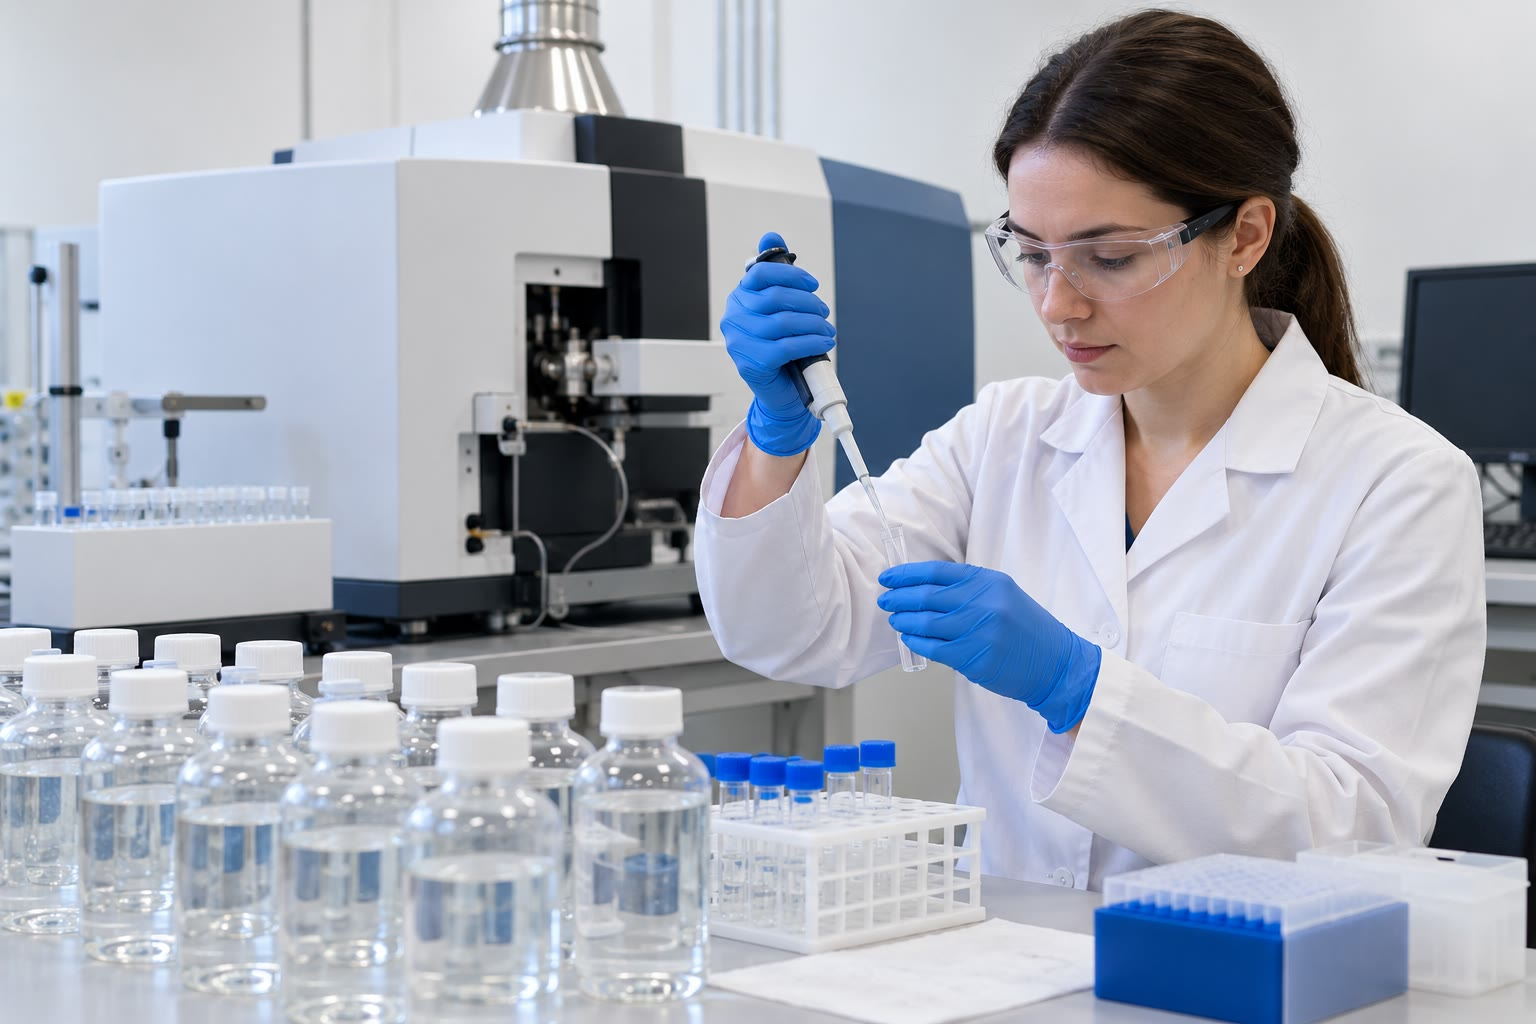
\includegraphics[width=0.56\linewidth]{images/book3/ai/b2-34-water-lab.jpg}

{\small 水质检测实验室：样品瓶、正在移液的技术人员，
后方为元素分析仪（示意）。}
\end{omfigure}

\begin{recall}
本科一年级分册：测量不确定度、标准不确定度、A 类和 B 类评定，
扩展不确定度、相对不确定度、两个值之间的归一化偏差 $z$，以及
承诺给出 $u(\bar x) = s/\sqrt n$ 的证明以及一般传递规则。第 1 册：
标准曲线。\Cref{ch:b2:mass-spec-atomic}：原子吸收。
\end{recall}

\section{重复测量}

重复测量时，结果会发生离散。将每个结果 $x_i$ 视为随机变量，
其均值为 $\mu$（即该方法的平均给出值），标准差为 $\sigma$；当许多
微小而相互独立的因素叠加时，结果服从正态（高斯）分布，约 68~\% 的结果
落在 $\mu \pm \sigma$ 之内，约 95~\% 落在 $\mu \pm 1.96\sigma$ 之内。

\begin{definition}[离散度]\label{def:b2:measurement-statistics:dispersion}
设 $n$ 个结果 $x_1, \dots, x_n$ 的均值为 $\bar x$，则称\emph{实验标准差
}\index{实验标准差}为 $s = \sqrt{\sum (x_i - \bar x)^2/(n-1)}$，它
估计 $\sigma$。称\emph{平均值的标准差}\index{平均值的标准差}
为 $\bar x$ 在多组、每组 $n$ 个结果上的标准差，其估计值为 $s/\sqrt n$。
\end{definition}

除数取 $n - 1$ 而非 $n$，是为了修正偏差取自 $\bar x$ 这一事实，
这一均值本身也由同一批数据算得，这使偏差略偏小：$n - 1$ 即
独立偏差的个数，即自由度。

\begin{theorem}[平均值的方差]\label{thm:b2:measurement-statistics:mean-variance}
若 $x_1, \dots, x_n$ 相互独立，且各自方差为 $\sigma^2$，则 $\operatorname{var}(\bar x) =
\sigma^2/n$，即平均值的标准差为 $\sigma/\sqrt n$。
\end{theorem}

\begin{proof}
对独立变量，和的方差等于各方差之和，且
$\operatorname{var}(cX) = c^2\operatorname{var}(X)$。于是 $\operatorname{var}(\bar x) =
\operatorname{var}\bigl(\tfrac1n\sum x_i\bigr) = \tfrac{1}{n^2}\sum\operatorname{var}(x_i) =
\tfrac{1}{n^2}\,n\sigma^2 = \sigma^2/n$。将 $\sigma$ 换为其估计值 $s$，得到
A 类标准不确定度 $u(\bar x) = s/\sqrt n$，已在本科一年级分册中承认。
\end{proof}

\section{置信区间}

\begin{definition}[置信区间]\label{def:b2:measurement-statistics:confidence}
称\emph{置信区间}\index{置信区间}为在\emph{置信水平}\index{置信水平}
$1 - \alpha$（常取 95~\%）下，由数据按某一规则算出的区间，该规则应用于
多组数据时，约 $1 - \alpha$ 的比例包含真值。对于 $n$ 个结果的均值，它为
$\bar x \pm t\,s/\sqrt n$，其中 $t$ 为\emph{学生 t 系数}\index{学生 t 系数}，
它取决于自由度 $n - 1$ 和该置信水平。
\end{definition}

\begin{proposition}[学生 t 分布]\label{prop:b2:measurement-statistics:student}
对于 $n$ 个独立的正态结果，$T = (\bar x - \mu)/(s/\sqrt n)$ 服从自由度为
$n - 1$ 的学生 t 分布，其密度正比于 $(1 + t^2/\nu)^{-(\nu+1)/2}$，其中
$\nu = n - 1$。它比正态分布更宽，且随 $n$ 增大趋于正态分布。
\end{proposition}

\admitted

用 $s$ 代替未知的 $\sigma$ 作除数，引入了 $s$ 本身的离散，
$n$ 较小时该离散较大，因此尾部更厚，系数大于 1.96。表中给出的是 95~\%
系数，由密度积分算得。

\begin{omfigure}
\begin{minipage}[c]{0.56\linewidth}
\begin{tikzpicture}
\begin{axis}[width=\linewidth, height=4.8cm, xmin=-5, xmax=5, ymin=0, ymax=0.43,
  xlabel={$t$}, ylabel={密度}, label style={font=\small}, tick label style={font=\scriptsize},
  legend style={font=\scriptsize, at={(0.98,0.98)}, anchor=north east}, legend cell align=left]
\addplot[omThm, thick] table[x=t, y=nu2] {figdata/out/bachelor-2-regression-c.dat};
\addplot[omMeth, thick] table[x=t, y=nu5] {figdata/out/bachelor-2-regression-c.dat};
\addplot[black, thick, dashed] table[x=t, y=normal] {figdata/out/bachelor-2-regression-c.dat};
\legend{$\nu = 2$, $\nu = 5$, 正态}
\end{axis}
\end{tikzpicture}
\end{minipage}\hfill
\begin{minipage}[c]{0.4\linewidth}\centering
\small
\begin{tabular}{rr}
\hline
$\nu = n - 1$ & $t$（95~\%） \\
\hline
1 & 12.706 \\
2 & 4.303 \\
3 & 3.182 \\
4 & 2.776 \\
5 & 2.571 \\
9 & 2.262 \\
20 & 2.086 \\
$\infty$ & 1.960 \\
\hline
\end{tabular}
\end{minipage}
\par\vspace{4pt}

{\small 自由度为 2 和 5 的学生 t 分布密度，与正态分布的对比，以及双侧
95~\% 系数，由密度积分算得（末行为正态分布）。}
% figdata: bachelor-2/regression.py parts c, e
\end{omfigure}

\begin{method}[均值的置信区间]\label{met:b2:measurement-statistics:confidence-interval}
\begin{enumerate}
  \item 计算 $\bar x$ 和 $s$，共 $n$ 个结果；检查有无结果明显偏离其余数据。
  \item 在所选置信水平下查 $t$，自由度 $\nu = n - 1$。
  \item 给出 $\bar x \pm t\,s/\sqrt n$，不确定度取一到两位有效数字，
        均值取相同的小数位。
  \item 与参考值 $x_{\mathrm{ref}}$ 比较时，计算 $|\bar x - x_{\mathrm{ref}}|/(s/\sqrt
        n)$：高于 $t$ 时，该置信水平下差异显著；低于此值时，数据未显示
        差异（这并不能证明不存在差异）。
\end{enumerate}
\end{method}

\section{不确定度的传播}

\begin{theorem}[不确定度传播定律]\label{thm:b2:measurement-statistics:propagation}
设 $y = f(x_1, \dots, x_n)$，其中各 $x_i$ 相互独立，标准不确定度 $u(x_i)$ 足够小，
使 $f$ 在其范围内近似线性，则
\begin{equation*}
u^2(y) = \sum_{i=1}^{n}\left(\frac{\partial f}{\partial x_i}\right)^2 u^2(x_i).
\end{equation*}
\end{theorem}

\begin{proof}
由泰勒一阶展开，$y - f(\mu_1, \dots, \mu_n) \approx \sum c_i(x_i - \mu_i)$，其中 $c_i = \partial
f/\partial x_i$ 在均值处取值。独立变量线性组合的方差为
$\sum c_i^2\operatorname{var}(x_i)$（见\cref{thm:b2:measurement-statistics:mean-variance}）；取
$\operatorname{var}(x_i) = u^2(x_i)$，即得所证结论。
\end{proof}

\begin{corollary}[和与积]\label{cor:b2:measurement-statistics:products}
对于和或差，标准不确定度按方和根合成：$u^2(x_1 \pm x_2) = u^2(x_1) +
u^2(x_2)$。对于积或商 $y = x_1^{a}x_2^{b}\cdots$，相对不确定度按
方和根合成，每项以其指数加权：$\bigl(u(y)/y\bigr)^2 = a^2\bigl(u(x_1)/x_1\bigr)^2 +
b^2\bigl(u(x_2)/x_2\bigr)^2 + \cdots$
\end{corollary}

\begin{proof}
对于和，偏导数为 $\pm1$。对于 $y = x_1^ax_2^b$，$\partial y/\partial x_1 =
a\,y/x_1$，$\partial y/\partial x_2 = b\,y/x_2$；由定理得 $u^2(y) = a^2y^2u^2(x_1)/x_1^2 +
b^2y^2u^2(x_2)/x_2^2$；两边除以 $y^2$。
\end{proof}

\begin{method}[传播不确定度]\label{met:b2:measurement-statistics:propagate}
\begin{enumerate}
  \item 将结果写成测得量的公式，列出每个输入量及其标准不确定度
        （A 类或 B 类评定）。
  \item 对积与商，用相对不确定度；对和与差，用绝对不确定度；
        其他情形取偏导数。
  \item 按方和根合成，找出主导项；改进其他各项是白费力气。
  \item 乘以包含因子（取 2，或在主导项来自较少次数的重复测量时取学生 $t$ 系数
        ），得扩展不确定度。
\end{enumerate}
\end{method}

\section{标准曲线}

\begin{definition}[标准曲线]\label{def:b2:measurement-statistics:calibration}
称\emph{标准曲线}\index{标准曲线}为联系仪器信号 $y$ 与
浓度 $x$ 的关系曲线，由已知浓度的标准溶液给出。\emph{最小二乘
直线}\index{最小二乘直线} $y = a + bx$ 是使 $S = \sum (y_i - a -
bx_i)^2$ 最小的直线；每个 $e_i = y_i - a - bx_i$ 称为\emph{残差}\index{残差}。
\end{definition}

\begin{theorem}[最小二乘直线]\label{thm:b2:measurement-statistics:least-squares}
记 $\bar x$、$\bar y$ 为均值，$S_{xx} = \sum(x_i - \bar x)^2$，$S_{xy} = \sum(x_i - \bar x)(y_i -
\bar y)$，则最小二乘直线的系数为
\begin{equation*}
b = \frac{S_{xy}}{S_{xx}}, \qquad a = \bar y - b\bar x.
\end{equation*}
\end{theorem}

\begin{proof}
$S$ 是关于 $a$ 与 $b$ 的二次函数，其偏导数在极小点处为零：
$\partial S/\partial a = -2\sum(y_i - a - bx_i) = 0$ 得 $a = \bar y - b\bar x$；代入
$\partial S/\partial b = -2\sum x_i(y_i - a - bx_i) = 0$ 得 $\sum x_i\bigl((y_i - \bar y) - b(x_i -
\bar x)\bigr) = 0$，即 $S_{xy} = bS_{xx}$（因 $\sum \bar x(y_i - \bar y) = \sum \bar x(x_i - \bar
x) = 0$）。二阶偏导数构成矩阵
\[\begin{pmatrix} 2n & 2\sum x_i\\ 2\sum x_i & 2\sum x_i^2\end{pmatrix},\]
其对角元为正，行列式 $4nS_{xx}$ 在 $x_i$ 不全
相等时为正，故驻点为极小点。
\end{proof}

\begin{proposition}[由标准曲线读取浓度]\label{prop:b2:measurement-statistics:interpolation}
对 $n$ 个标准样品，残差标准差 $s_{y/x} = \sqrt{\sum e_i^2/(n-2)}$，若一个样品
测量 $m$ 次，平均信号为 $\bar y_0$，则其 $x_0 = (\bar y_0 - a)/b$，标准差为
\begin{equation*}
s_{x_0} = \frac{s_{y/x}}{b}\sqrt{\frac1m + \frac1n + \frac{(\bar y_0 - \bar y)^2}{b^2S_{xx}}},
\end{equation*}
应配合学生 $t$ 系数使用，自由度为 $n - 2$。
\end{proposition}

\admitted

根号下的三项分别是样品读数的散布、直线截距的不确定度
以及斜率的不确定度；最后一项在标准曲线范围的中心处为零，这正是
读取样品最可靠之处。

\begin{omfigure}
\begin{tikzpicture}
\begin{axis}[width=0.5\linewidth, height=5cm, xmin=-1, xmax=22, ymin=0, ymax=0.22,
  xlabel={铅 (\unit{\micro g/L})}, ylabel={吸光度}, label style={font=\small},
  tick label style={font=\scriptsize}, scaled y ticks=false,
  yticklabel style={/pgf/number format/fixed, /pgf/number format/precision=2}]
\addplot[omDef, thick] table[x=x, y=line] {figdata/out/bachelor-2-regression-b.dat};
\addplot[only marks, mark=*, mark size=1.8pt, omThm] table[x=x, y=A] {figdata/out/bachelor-2-regression-a.dat};
\end{axis}
\end{tikzpicture}\hfill
\begin{tikzpicture}
\begin{axis}[width=0.5\linewidth, height=5cm, xmin=-1, xmax=22, ymin=-0.002, ymax=0.002,
  xlabel={铅 (\unit{\micro g/L})}, ylabel={残差}, label style={font=\small},
  tick label style={font=\scriptsize}, scaled y ticks=false, ycomb,
  yticklabel style={/pgf/number format/fixed, /pgf/number format/precision=3},
  extra y ticks={0}, extra y tick style={grid=major, grid style={black!50}}]
\addplot[omThm, thick, mark=*, mark size=1.6pt] table[x=x, y=res] {figdata/out/bachelor-2-regression-a.dat};
\end{axis}
\end{tikzpicture}

{\small 石墨炉原子吸收法标定铅，波长 \qty{283.3}{nm}（练习数据，
用于本题）。左图：五个标准样品及最小二乘直线。右图：残差，数值很小，
且无规律，直线拟合是合适的。}
% figdata: bachelor-2/regression.py parts a, b
% ledger: asd:Pb283
\end{omfigure}

\begin{method}[标定]\label{met:b2:measurement-statistics:calibrate}
\begin{enumerate}
  \item 配制至少五个覆盖预期范围的标准样品，基体与样品相同，
        并配制一个空白。
  \item 拟合最小二乘直线，并作残差图。残差呈曲线形态说明响应不是
        线性的：缩小范围或拟合曲线。单个残差很大则提示某个标准样品有问题。
  \item 测定样品，最好取在范围中部附近，并作平行测定；计算 $x_0$ 和
        $s_{x_0}$。
  \item 对每一次稀释进行校正后报告 $x_0 \pm t\,s_{x_0}$，若稀释的传递
        不确定度不可忽略，则一并计入。
\end{enumerate}
\end{method}

\begin{definition}[标准加入法]\label{def:b2:measurement-statistics:standard-addition}
在\emph{标准加入法}\index{标准加入法}中，将已知量的待测物加入到等量的样品本身中，
以信号对所加入的浓度作图，
样品中待测物的浓度为直线外推至信号为零时与横轴交点
到原点的距离，即 $a/b$。
\end{definition}

\begin{method}[标准加入法]\label{met:b2:measurement-statistics:standard-addition}
\begin{enumerate}
  \item 当样品基体会改变响应时使用（如盐类、酸类、有机物），
        否则用纯水配制的标准样品会给出错误的斜率。
  \item 取等量样品，分别加入递增的已知量，全部稀释至相同体积后测量。
  \item 拟合直线；被测溶液中的浓度为 $a/b$，并校正稀释倍数。
  \item 响应须从零开始呈线性：需检查残差。
\end{enumerate}
\end{method}

\begin{omfigure}
\begin{tikzpicture}
\begin{axis}[width=0.62\linewidth, height=5cm, xmin=-4, xmax=7, ymin=0, ymax=0.42,
  xlabel={加入浓度 (\unit{mg/L})}, ylabel={吸光度}, label style={font=\small},
  tick label style={font=\scriptsize}, axis lines=left, scaled y ticks=false,
  yticklabel style={/pgf/number format/fixed, /pgf/number format/precision=1}]
\draw[black!40] (axis cs:0,0) -- (axis cs:0,0.42);
\addplot[omDef, thick, densely dashed] table[x=x, y=line] {figdata/out/bachelor-2-regression-d-line.dat};
\addplot[only marks, mark=*, mark size=1.8pt, omThm] table[x=x, y=A] {figdata/out/bachelor-2-regression-d.dat};
\draw[<->, omMeth, thick] (axis cs:-3.11,0.06) -- (axis cs:0,0.06); \node[omMeth, below, font=\scriptsize] at (axis cs:-0.8,0.055) {$a/b$};
\end{axis}
\end{tikzpicture}

{\small 标准加入法（练习数据）：加入 0、2、4 和
\qty{6}{mg/L} 待测物的样品吸光度。直线与零信号处的交点为 \qty{-3.11}{mg/L}：被测溶液
含 \qty{3.11}{mg/L}。}
% figdata: bachelor-2/regression.py part d
\end{omfigure}

\section{检出、定量与方法验证}

\begin{definition}[检出限与定量限]\label{def:b2:measurement-statistics:limits}
方法的\emph{检出限}\index{检出限}是指：能与空白信号相区分的最小浓度，
且误检风险为给定的较小值；
\emph{定量限}\index{定量限}是指能以可接受的相对不确定度测定的
最小浓度。
\end{definition}

\begin{proposition}[常用估计]\label{prop:b2:measurement-statistics:lod}
设 $s_{\mathrm{blank}}$ 为重复测定空白信号的标准差，$b$ 为
标准曲线的斜率，则 $x_{\mathrm{LOD}} \approx 3s_{\mathrm{blank}}/b$，$x_{\mathrm{LOQ}} \approx
10s_{\mathrm{blank}}/b$。
\end{proposition}

\begin{proof}[论证]
若空白信号服从标准差为 $s_{\mathrm{blank}}$ 的正态分布，则空白信号
高出其均值超过 $3s_{\mathrm{blank}}$ 的概率约为 0.13~\%（正态分布超过
3 个标准差的单侧尾部）：高于该阈值的信号被判为“已检出”，几乎不会把空白误认作
样品。高于空白 $10s_{\mathrm{blank}}$ 的信号，其相对标准差约为
10~\%，这是定量结果通常采用的阈值。除以 $b$ 即可将信号换算为
浓度。
\end{proof}

\begin{definition}[方法验证]\label{def:b2:measurement-statistics:validation}
\emph{正确度}\index{正确度}是大量结果的均值与真值的接近程度；
二者之差即为\emph{偏倚}\index{偏倚}。\emph{精密度}\index{精密度}是
独立结果彼此之间的接近程度，以标准差表示：
\emph{重复性}\index{重复性}是指相同条件（同一操作者、同一仪器、
同一实验室、短时间内）下的一致程度，\emph{再现性}\index{再现性}则是条件改变
（不同实验室）时的一致程度。\emph{方法验证}\index{方法验证}是一组实验，
用以确定某一方法的正确度、精密度、线性与范围，以及其检出限
与定量限。
\end{definition}

正确度可通过与有证标准物质比对或加标进行检验；精密度则通过
同一实验室的平行测定及实验室间比对来检验。一种方法可以精密但有偏倚，
即各结果彼此接近，却都是错的：精密度并不能证明正确度。

\begin{history}[学生，1908]
\begin{minipage}[t]{0.17\linewidth}
\vspace{0pt}
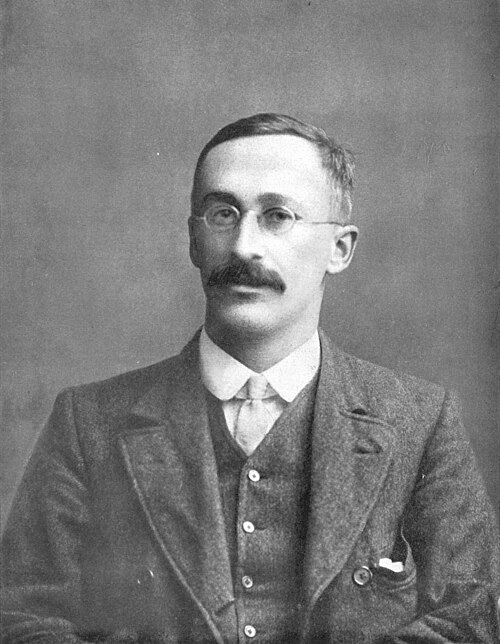
\includegraphics[width=\linewidth]{images/book3/gosset.jpg}
\end{minipage}\hfill
\begin{minipage}[t]{0.79\linewidth}
\vspace{0pt}
威廉·西利·戈塞特是一家酿酒厂的化学家，需要根据极少的样品判断原料，
样本量远不足以套用正态分布。1908 年，他发表了样本均值除以样本
标准差的分布，并以笔名“学生”发表，因为雇主不允许员工以真名发表
论文。学生分布律在分析人员每次由三至四次
平行测定给出区间时都会用到。（照片，1908 年：公有领域；维基共享资源。）
\end{minipage}
\end{history}

\section{练习}

\begin{exercise}[$\star$]\label{exo:b2:measurement-statistics:1}
五次滴定得到 12.45、12.50、12.48、12.52 和 \qty{12.46}{mL}。求其平均值、
实验标准差和平均值的标准差。
\end{exercise}

\begin{exercise}[$\star$]\label{exo:b2:measurement-statistics:2}
求练习~1 中平均值的 95~\% 置信区间。
\end{exercise}

\begin{exercise}[$\star$]\label{exo:b2:measurement-statistics:3}
将 $m = \qty{0.5000}{g}$（$u = \qty{0.0002}{g}$）的固体溶于
$V = \qty{250.0}{mL}$（$u = \qty{0.15}{mL}$）的容量瓶中，配成溶液。求 $c = m/(MV)$ 的相对标准不确定度，
摩尔质量可视为足够精确。
\end{exercise}

\begin{exercise}[$\star$]\label{exo:b2:measurement-statistics:4}
求数据点 $(0, 0.02)$、$(1, 0.21)$、$(2, 0.39)$、$(3, 0.62)$ 的最小二乘直线。
\end{exercise}

\begin{exercise}[$\star\star$]\label{exo:b2:measurement-statistics:5}
一份有证参考溶液含某元素 \qty{10.00}{mg/L}。五次分析的平均值为
\qty{10.12}{mg/L}，$s = \qty{0.08}{mg/L}$。在 95~\% 水平上，该方法是否存在偏倚？
\end{exercise}

\begin{exercise}[$\star\star$]\label{exo:b2:measurement-statistics:6}
已知水合氢离子浓度的相对标准不确定度为 2~\%。
pH 的标准不确定度是多少？
\end{exercise}

\begin{exercise}[$\star\star$]\label{exo:b2:measurement-statistics:7}
十个空白样品的 $s = 0.0012$ 吸光度单位；标准曲线的斜率为 \qty{0.0098}{L/\micro g}。
估算检出限和定量限。
\end{exercise}

\begin{exercise}[$\star\star$]\label{exo:b2:measurement-statistics:8}
图中标准加入法实验的四份溶液，
均取 \qty{10.0}{mL} 样品稀释至 \qty{50.0}{mL} 配制而成。求样品中的浓度。
\end{exercise}

\begin{exercise}[$\star\star$]\label{exo:b2:measurement-statistics:9}
在一项实验室间比对中，每个实验室对自身平行测定得到的 $s = \qty{0.05}{mg/L}$，但
不同实验室结果的散布为 $s = \qty{0.15}{mg/L}$。指出这两个量，并
说明二者的区别。
\end{exercise}

\begin{exercise}[$\star\star\star$]\label{exo:b2:measurement-statistics:10}
证明最小二乘直线过点 $(\bar x, \bar y)$，且其残差之和为零。
\end{exercise}

\begin{exercise}[$\star\star\star$]\label{exo:b2:measurement-statistics:11}
将母液稀释一百倍，可一步完成（取 \qty{1.000}{mL} 稀释至 \qty{100.0}{mL}），或
分两步十倍稀释（两次均取 \qty{10.00}{mL} 稀释至 \qty{100.0}{mL}）。标准不确定度：1 mL
移液管 \qty{0.006}{mL}，10 mL 移液管 \qty{0.02}{mL}，100 mL 容量瓶 \qty{0.08}{mL}（练习数据）。
哪一种途径更精密？
\end{exercise}

\begin{exercise}[$\star\star\star$]\label{exo:b2:measurement-statistics:12}
开篇所述两个实验室报告的结果为 9.6 和 \qty{11.2}{\micro g/L}，标准不确定度分别为
0.4 和 \qty{0.5}{\micro g/L}（练习数据）。两者的结果是否相容？各实验室的结果对
准则值说明了什么？
\end{exercise}

\section{问题：自来水中的铅}

\begin{problem}[{周末问题——最小二乘标准曲线的原子吸收校准，
样品浓度及其置信区间，稀释及检出限、定量限，以及
对照准则值的结论}]
\label{pb:b2:measurement-statistics:1}
练习数据。铅采用石墨炉原子吸收法，在 \qty{283.3}{nm} 处测定。标准溶液
（\unit{\micro g/L}；吸光度）：0.0；0.003，5.0；0.051，10.0；0.101，15.0；0.148，20.0；0.199。
自来水（\qty{50.0}{mL}）以 \qty{0.50}{mL} 硝酸酸化；该溶液的三次读数为
0.104、0.098 和 0.101。十个空白样品：0.002、0.004、0.003、0.001、0.003、0.005、0.002、
0.003、0.004、0.003。各体积的标准不确定度：50.0 mL 为 \qty{0.03}{mL}，
0.50 mL 为 \qty{0.005}{mL}。准则值：\qty{10}{\micro g/L}。
% ledger: who:lead, asd:Pb283

\medskip
\noindent\textbf{第一部分——标准曲线。}
\begin{enumerate}
  \item 为何标准溶液要与样品使用相同的硝酸配制？
  \item 求最小二乘直线的斜率和截距。
  \item 求五个残差。
  \item 残差是否呈现规律？并据此判断线性。
  \item 求 $s_{y/x}$。
  \item 截距为何不为零？
  \item 斜率表示什么？
\end{enumerate}

\medskip
\noindent\textbf{第二部分——样品测定。}
\begin{enumerate}[resume]
  \item 求三次读数的平均值和标准差。
  \item 求所测溶液中铅的浓度。
  \item 求 $s_{x_0}$。
  \item 自由度是多少，应取哪个学生 t 系数？
  \item 给出所测溶液中浓度的 95~\% 置信区间。
  \item 为何要将样品读数三次而非一次？
\end{enumerate}

\medskip
\noindent\textbf{第三部分——稀释与检出限和定量限。}
\begin{enumerate}[resume]
  \item 求稀释倍数及自来水中的浓度。
  \item 将两个体积的不确定度传递到稀释倍数上。
  \item 与标准曲线的不确定度相比，该项是否显著？
  \item 求空白的标准差及检出限。
  \item 求定量限。
  \item 样品浓度是否高于定量限？
\end{enumerate}

\medskip
\noindent\textbf{第四部分——结论。}
\begin{enumerate}[resume]
  \item 该区间是否包含准则值？
  \item 若仅读数一次得到 0.104，会得出什么结论？
  \item 此处“95~\% 置信”意味着什么？
  \item 实验室如何能更有把握地作出判断？
  \item 如何检验该方法不存在偏倚？
  \item 该准则值是暂定的，“以处理效果和分析可达性为依据
        ”。第二个理由在本题中意味着什么？
  \item 给出自来水中铅的浓度及其 95~\% 置信区间，并与
        \qty{10}{\micro g/L} 比较。
\end{enumerate}
\end{problem}
